\documentclass{article}
\usepackage{amsmath}
\usepackage{amsfonts}
\usepackage{geometry}
\usepackage{booktabs}
\usepackage{graphicx}
\usepackage{tikz}
\usetikzlibrary{arrows.meta}

\geometry{a4paper, margin=1in}

\begin{document}

\title{Kinematics Part II: 2D Motion \& Projectiles}
\author{}
\date{}
\maketitle

\section{Vector Foundations}

In 2D kinematics, physical quantities are no longer just ``left/right or upward/downward.'' Therefore, we must introduce vectors to describe both magnitude and direction.

\subsection{Vector Basics \& Addition}
A vector $\vec{A}$ can be represented by an arrow. The length represents the \textbf{magnitude}, and the tip points in the \textbf{direction}.

\subsubsection{Geometric Addition (Tip-to-Tail)}

\begin{center}
  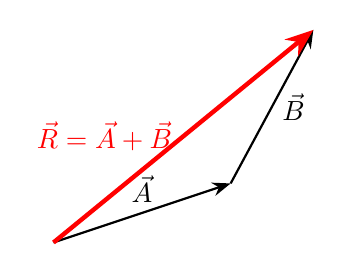
\begin{tikzpicture}[>=Stealth, scale=1.5]
    \draw[->, thick] (0,0) -- (1.5,0.5) node[midway, above] {$\vec{A}$};
    \draw[->, thick] (1.5,0.5) -- (2.2,1.8) node[midway, right] {$\vec{B}$};
    \draw[->, ultra thick, red] (0,0) -- (2.2,1.8) node[midway, left] {$\vec{R} = \vec{A} + \vec{B}$};
  \end{tikzpicture}
\end{center}

To find the resultant vector $\vec{R} = \vec{A} + \vec{B}$:
\begin{enumerate}
  \item Draw vector $\vec{A}$.
  \item Place the tail of $\vec{B}$ at the tip of $\vec{A}$.
  \item $\vec{R}$ is the vector drawn from the start of $\vec{A}$ to the end of $\vec{B}$.
\end{enumerate}

\subsubsection{Vector Subtraction}

\begin{center}
  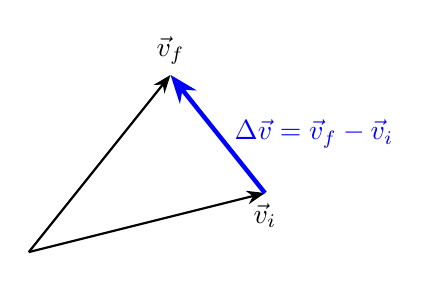
\begin{tikzpicture}[>=Stealth, scale=1.5]
    \draw[->, thick] (0,0) -- (2,0.5) node[below] {$\vec{v}_i$};
    \draw[->, thick] (0,0) -- (1.2,1.5) node[above] {$\vec{v}_f$};

    \draw[->, ultra thick, blue] (2,0.5) -- (1.2,1.5) node[midway, right, xshift=2pt] {$\Delta \vec{v} = \vec{v}_f - \vec{v}_i$};
  \end{tikzpicture}
\end{center}

Subtracting a vector is the same as adding its opposite: $\vec{A} - \vec{B} = \vec{A} + (-\vec{B})$. In kinematics, this is essential for calculating \textbf{change in velocity} ($\Delta \vec{v} = \vec{v}_f - \vec{v}_i$).

\subsection{Trigonometric Decomposition}

\begin{center}
  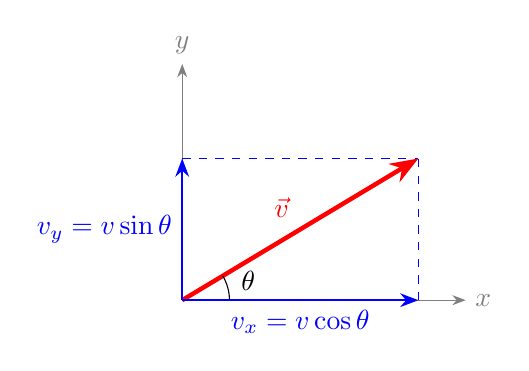
\begin{tikzpicture}[>=Stealth, scale=1.2]
    \draw[->, thin, gray] (0,0) -- (3,0) node[right] {$x$};
    \draw[->, thin, gray] (0,0) -- (0,2.5) node[above] {$y$};

    \draw[dashed, blue] (2.5,0) -- (2.5,1.5);
    \draw[dashed, blue] (0,1.5) -- (2.5,1.5);

    \draw[->, ultra thick, red] (0,0) -- (2.5,1.5) node[midway, above left] {$\vec{v}$};

    \draw[->, thick, blue] (0,0) -- (2.5,0) node[midway, below] {$v_x = v\cos\theta$};
    \draw[->, thick, blue] (0,0) -- (0,1.5) node[midway, left] {$v_y = v\sin\theta$};

    \draw (0.5,0) arc (0:31:0.5);
    \node at (0.7,0.2) {$\theta$};
  \end{tikzpicture}
\end{center}

To use our 1D kinematic equations, we must "break" a diagonal vector into two perpendicular components.

\begin{itemize}
  \item \textbf{Horizontal Component ($x$):} $v_x = v \cos \theta$
  \item \textbf{Vertical Component ($y$):} $v_y = v \sin \theta$
\end{itemize}
\textit{Note: $\theta$ is the angle measured from the horizontal axis.}

\subsection{Vector Composition (The "Rebuild")}

\begin{center}
  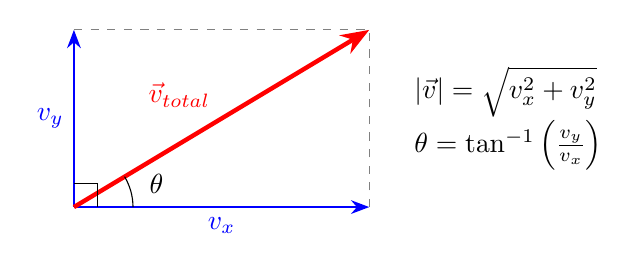
\begin{tikzpicture}[>=Stealth, scale=1.5]
    % 定义坐标点
    \coordinate (O) at (0,0);
    \coordinate (X) at (2.5,0);
    \coordinate (Y) at (0,1.5);
    \coordinate (P) at (2.5,1.5);

    % 画虚线辅助线（形成矩形）
    \draw[dashed, gray] (X) -- (P);
    \draw[dashed, gray] (Y) -- (P);

    % 画分量矢量
    \draw[->, thick, blue] (O) -- (X) node[midway, below] {$v_x$};
    \draw[->, thick, blue] (O) -- (Y) node[midway, left] {$v_y$};

    % 画合成后的合矢量
    \draw[->, ultra thick, red] (O) -- (P) node[midway, above left] {$\vec{v}_{total}$};

    % 标注直角符号
    \draw[thin] (0.2,0) -- (0.2,0.2) -- (0,0.2);

    % 标注角度 theta
    \draw (0.5,0) arc (0:31:0.5);
    \node at (0.7,0.2) {$\theta$};

    % 旁边的公式标注（可选）
    \node[right, align=left] at (2.8, 0.75) {
      $|\vec{v}| = \sqrt{v_x^2 + v_y^2}$ \\
      $\theta = \tan^{-1} \left( \frac{v_y}{v_x} \right)$
    };
  \end{tikzpicture}
\end{center}
After solving for the final horizontal velocity ($v_{fx}$) and vertical velocity ($v_{fy}$), we often need to find the actual \textbf{final speed} and \textbf{impact angle}.

\begin{itemize}
  \item \textbf{Magnitude (Pythagorean Theorem):}
    \begin{equation}
      |\vec{v}| = \sqrt{v_x^2 + v_y^2}
    \end{equation}
  \item \textbf{Direction (Inverse Tangent):}
    \begin{equation}
      \theta = \tan^{-1} \left( \frac{|v_y|}{|v_x|} \right)
    \end{equation}
\end{itemize}

\subsection{Relative Motion (Optional/Advanced)}
When an object moves within a moving medium (e.g., a plane in wind, a boat in a river), we use vector addition:
\begin{equation}
  \vec{v}_{\text{object relative to ground}} = \vec{v}_{\text{object relative to medium}} + \vec{v}_{\text{medium relative to ground}}
\end{equation}

\newpage
\section{The Principle of Independence}

The fundamental rule of 2D kinematics is: \textbf{motion in the $x$ and $y$ directions is independent.}
\begin{quote}
  An object's horizontal velocity does not affect its vertical velocity or acceleration, and vice versa.
\end{quote}

\subsection{What ``Independent'' Really Means}
Independence does \textbf{not} mean the object is doing two separate trips. It means that, for projectile motion (neglecting air resistance):
\begin{itemize}
  \item The \textbf{horizontal} motion is constant-velocity motion because $a_x = 0$.
  \item The \textbf{vertical} motion is free-fall motion because $a_y = -g$.
  \item The \textbf{same time interval} $\Delta t$ applies to both directions.
\end{itemize}

\subsection{Two Separate Kinematics ``Tracks''}
You can run the 1D kinematic equations twice:
\begin{align}
  \Delta x &= v_{ix}\,\Delta t + \tfrac{1}{2}a_x(\Delta t)^2 \qquad (a_x = 0) \\
  \Delta y &= v_{iy}\,\Delta t + \tfrac{1}{2}a_y(\Delta t)^2 \qquad (a_y = -g)
\end{align}
Even though the object follows a \emph{curved} path, each component still follows a 1D rule.

\subsection{Common Consequences (Projectiles)}
\begin{itemize}
  \item Changing $v_{ix}$ changes the \textbf{range} (how far it goes) but does \textbf{not} change the time to fall if $\Delta y$ and $v_{iy}$ are unchanged.
  \item Changing $v_{iy}$ changes the \textbf{time in the air} and \textbf{maximum height}, but does \textbf{not} change the fact that $v_x$ stays constant (again, if air resistance is neglected).
  \item The vertical velocity changes linearly with time:
    \begin{equation}
      v_y = v_{iy} - g\,\Delta t
    \end{equation}
\end{itemize}

\subsection{Why the Path Is a Parabola (Optional)}
From $\Delta x = v_{ix}\Delta t$, we get $\Delta t = \frac{\Delta x}{v_{ix}}$. Substitute into the $y$ equation:
\begin{equation}
  \Delta y = \left(\frac{v_{iy}}{v_{ix}}\right)\Delta x - \frac{g}{2v_{ix}^2}(\Delta x)^2,
\end{equation}
which is a quadratic in $\Delta x$, so the trajectory is parabolic.

\newpage
\section{Projectile Motion}
A projectile is an object moving through the air, acted upon only by gravity ($g \approx 9.8 \, \text{m/s}^2$ downward).

\subsection{Model Assumptions (Read This First)}
Unless stated otherwise, projectile-motion problems in this unit assume:
\begin{itemize}
  \item \textbf{No air resistance} (so the only force is gravity).
  \item \textbf{Constant gravitational acceleration} near Earth's surface.
  \item \textbf{A consistent sign convention} (here: upward is $+y$, so $a_y=-g$).
\end{itemize}
If air resistance matters, then typically $a_x \neq 0$ and $v_x$ will \emph{not} remain constant.

\begin{center}
  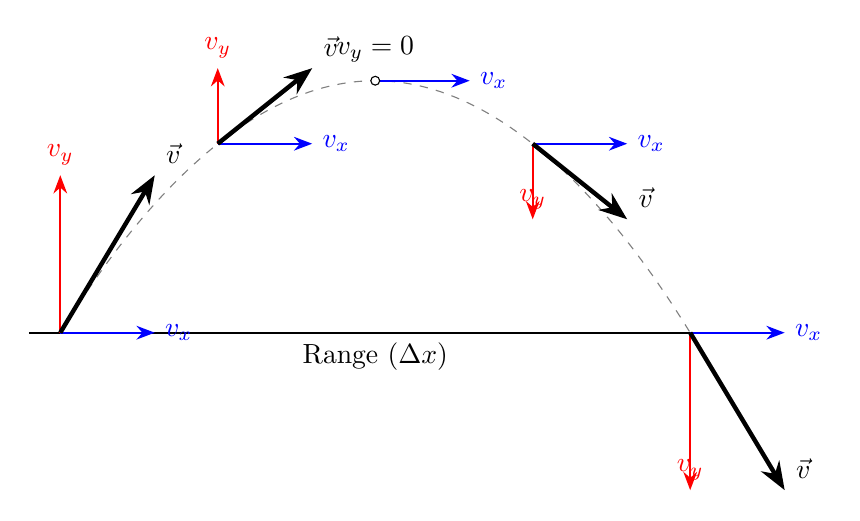
\begin{tikzpicture}[>=Stealth, scale=0.8]
    % 地面
    \draw[thick] (-0.5,0) -- (10.5,0);

    % 抛物线轨迹
    \draw[dashed, gray] (0,0) parabola bend (5,4) (10,0);

    % 定义绘制矢量的命令: \drawVectors{x}{y}{label}
    \newcommand{\drawVectors}[3]{
      \draw[->, blue, thick] (#1,#2) -- ++(1.5,0) node[right] {$v_x$}; % 水平恒定
      \draw[->, red, thick] (#1,#2) -- ++(0,#3) node[above] {$v_y$}; % 垂直变化
      \draw[->, black, ultra thick] (#1,#2) -- ++(1.5,#3) node[above right] {$\vec{v}$}; % 合速度
    }

    % 起点
    \drawVectors{0}{0}{2.5}
    % 上升中 (point lies on the parabola y = -0.16(x-5)^2 + 4)
    \drawVectors{2.5}{3.0}{1.2}
    % 最高点 (vy=0)
    \draw[->, blue, thick] (5,4) -- ++(1.5,0) node[right] {$v_x$};
    \draw[fill=white] (5,4) circle (2pt) node[above=3pt] {$v_y=0$};
    % 下降中
    \drawVectors{7.5}{3}{-1.2}
    % 落地前
    \drawVectors{10}{0}{-2.5}

    \node[below] at (5,0) {Range ($\Delta x$)};
  \end{tikzpicture}
\end{center}

\subsection{The Kinematic Split}
To solve 2D problems, you must maintain two separate inventories of variables. \textbf{Time ($\Delta t$)} is the only variable that is shared between both dimensions.

AGAIN: \textbf{Time ($\Delta t$)} is the only variable that is shared between both dimensions.

\begin{table}[h]
  \centering
  \caption{X vs Y Variables (Standard Projectile)}
  \begin{tabular}{lll}
    \toprule
    \textbf{Variable} & \textbf{Horizontal ($x$)} & \textbf{Vertical ($y$)} \\ \midrule
    Acceleration ($a$) & $a_x = 0$ (Constant Velocity) & $a_y = -g$ (Free Fall) \\
    Initial Velocity & $v_{ix} = v_i \cos \theta$ & $v_{iy} = v_i \sin \theta$ \\
    Displacement & $\Delta x$ (Range) & $\Delta y$ (Height/Vertical drop) \\
    Basic Equation & $\Delta x = v_{ix} \Delta t$ & $\Delta y = v_{iy} \Delta t + \frac{1}{2} a_y (\Delta t)^2$ \\ \bottomrule
  \end{tabular}
\end{table}

\newpage

\section{Key Concepts \& "Hidden" Information}
\begin{enumerate}
  \item \textbf{The Peak (Highest Point):} At the very top of the trajectory, the vertical velocity is zero ($v_{fy} = 0$), but the horizontal velocity $v_x$ remains $v_{ix}$.
  \item \textbf{Symmetry:} If a projectile starts and lands at the same height:
    \begin{itemize}
      \item Time to peak = $\frac{1}{2}$ Total flight time.
      \item Final speed = Initial speed (but velocity direction is different).
    \end{itemize}
  \item \textbf{Secondary Conclusions (Useful ``Shortcuts''):}
    \begin{itemize}
      \item \textbf{Time to peak:} $t_{\text{up}} = \dfrac{v_{iy}}{g}$ (only when the projectile rises to a point where $v_y=0$).
      \item \textbf{Maximum height above launch point:} $\Delta y_{\max} = \dfrac{v_{iy}^2}{2g}$.
      \item \textbf{Total flight time (same launch/landing height):} $T = \dfrac{2v_{iy}}{g}$.
      \item \textbf{Range (same launch/landing height):} $R = v_{ix}T = \dfrac{2v_{ix}v_{iy}}{g} = \dfrac{v_i^2\sin(2\theta)}{g}$.
    \end{itemize}

\end{enumerate}

\newpage
\section{The 2D Five-Step Method}
\begin{enumerate}
  \item \textbf{Resolve $v_i$:} Use $\sin$ and $\cos$ to find $v_{ix}$ and $v_{iy}$.
  \item \textbf{Two-Column Inventory:} Draw a table for $x$ and $y$ variables.
  \item \textbf{The Time Bridge:} Identify which dimension has enough info to find $\Delta t$.
    \begin{itemize}
      \item Most often, solve for $\Delta t$ using the $y$ direction (since $a_y=-g$ is known).
      \item Then use that same $\Delta t$ in the $x$ direction to find $\Delta x$ (range) or other horizontal quantities.
    \end{itemize}
  \item \textbf{Solve for the Unknown:} Use the $\Delta t$ to find the required value in the other dimension.
  \item \textbf{Recombine (If needed):} If the question asks for "final velocity," use Pythagoras to combine $v_{fx}$ and $v_{fy}$.
\end{enumerate}

\end{document}
